\documentclass[11pt,t]{beamer}
\usetheme[kulak]{kuleuven2}	%THEME OPTIONS for LOGO: kul (default), kulak, lrd,    ; OPTIONS for TITLE PAGE: normal (default), sedes


%%% OTHER SETTINGS
\usefonttheme[onlymath]{serif}			% math font with serifs, delete to make it sans-serif
\setbeamertemplate{footline}[body] 		% delete this line to remove footline bar on all frames
\usepackage[orientation=landscape,size=custom,width=16,height=9,scale=0.5,debug]{beamerposter}


%%% ADDED PACKAGES:
\usepackage[english]{babel}
\usepackage{amsfonts}
\usepackage{amssymb}

\newcommand{\rood}[1]{\color{red}#1\color{black}}


%%% TITLE PAGE INFO:
\title[A\&D Chapter 18: B-trees]{Algorithms and Data Structures} %[]] will appear in footline
\subtitle{Chapter 18: B-trees\\(based on book “Introduction to Algorithms” of Cormen et al.)}

\author{Vincent Van Schependom}
\institute{KU Leuven Campus Kulak Kortrijk}
\date{Academic year 2024--2025}




\begin{document}
	\csname beamer@calculateheadfoot\endcsname %recalculate head and foot dimension


	%%
	%%  0. TITLE PAGE and TABLE OF CONTENT
	%%
	% Title page
	\begin{frame}[plain,noframenumbering]
		\titlepage
	\end{frame}


	% Table of Contents
	\begin{frame}{Outline}
		\hfill	{\large \parbox{.961\textwidth}{\tableofcontents[hideothersubsections]}}
	\end{frame}

	\section{Definition of a B-tree}

	\begin{frame}{Definition of a B-tree}
		\begin{itemize}[<+->]
			\item Rooted tree with root \(T.root\)
			\item Self-balancing, just like red-black trees.
			\item All leaves have the same depth, i.e. the tree's height \(h\).
			\item Every node \(x\) has \underline{\(x.n\) keys}, stored in monotonically increasing order: \begin{align*}
				{x.key_1 \leq x.key_2 \leq \ldots \leq x.key_{x.n}}
			\end{align*}
			\item Each internal node contains \underline{\(x.n+1\) pointers to its children}:
			\begin{align*}
				x.c_1, x.c_2, \ldots, x.c_{x.n+1}
			\end{align*}
		\end{itemize}
	\end{frame}

	\begin{frame}{Definition of a B-tree}
		\begin{itemize}
			\item Rooted tree with root \(T.root\)
			\item Self-balancing, just like red-black trees.
			\item All leaves have the same depth, i.e. the tree's height \(h\).
			\item Every node \(x\) has \(\rood{x.n}\) \rood{keys}, stored in monotonically increasing order: \begin{align*}
				{x.key_1 \leq x.key_2 \leq \ldots \leq x.key_{x.n}}
			\end{align*}
			\item Each internal node contains \(\rood{x.n+1}\) pointers to its \rood{children}:
			\begin{align*}
				x.c_1, x.c_2, \ldots, x.c_{x.n+1}
			\end{align*}
			\item Main concept \(\rightarrow\) remember well
		\end{itemize}
	\end{frame}

	\begin{frame}{Example of a B-tree}
		\centering
		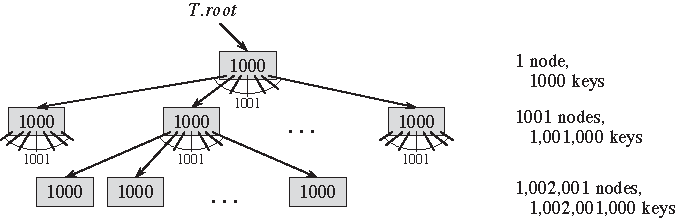
\includegraphics{images/nodes_keys}
		\vspace{0.5cm}
		\begin{itemize}[<+->]
			\item Every node \(x\) has \(x.n=1000\) keys \(x.key_i\).
			\item Each internal node \(x\) has \(x.n+1=1001\) pointers to its children \(x.c_i\).
		\end{itemize}
	\end{frame}

	\begin{frame}{Key ordering}
		\begin{itemize}[<+->]
			\item The keys \(x.key_i\) separate the ranges of keys stored in each subtree. \begin{itemize}[<+->]
				\item Let \(k_i\) be any key stored in the subtree with root \(x.c_i\)
%				\begin{itemize}
%					\item \(k_i\) is one of the keys of child \(x.c_i\) of node \(x\)
%					\item \(k_i\) is one of the keys of a descendant of child \(x.c_i\) of node \(x\)
%				\end{itemize}
			\end{itemize}
			\onslide<+-> \begin{align*}
				k_1 \leq x.key_1 \leq k_2 \leq x.key_2 \leq \ldots \leq x.key_{x.n} \leq k_{x.n+1}
			\end{align*} \vspace{-0.8cm}
			\item Example:
		\end{itemize}
		\centering
		\onslide<4>{ 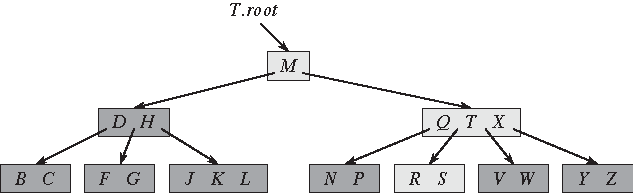
\includegraphics[width=.7\textwidth]{images/letters}}
		\vspace{0.5cm}
	\end{frame}

	\begin{frame}{Minimum degree}
		\begin{itemize}[<+->]
			\item Nodes have lower and upper bounds on the number of keys they can contain.
			\item Expressed in terms of a fixed integer \(t \geq 2\), called the \textit{minimum degree}
			\item Lower bound: \begin{itemize}[<+->\enspace]
				\item Every node other than the root must have \underline{at least \(t-1\) keys}.
				\item So, how many children does an internal node need at least? \onslide<+-> \(t\) children.
				\item If the tree is nonempty, the root must have at least one key.
			\end{itemize}
			\item Upper bound: \begin{itemize}[<+->\enspace]
				\item Every node may contain \underline{at most \(2t-1\) keys}.
				\item So, how many children can an internal node have at most? \onslide<+-> \(2t\) children.
				\item We say that a node is \textit{full} if it contains exactly \(2t-1\) keys.
			\end{itemize}
%			\item Why isn’t a minimum degree of \(t=1\) allowed? \onslide<+-> Trivial.
		\end{itemize}
	\end{frame}

	\section{Use-cases}

	\begin{frame}{Quick SOCS recap}
		\begin{itemize}[<+->]
			\item Computer systems use a hierarchy of memory technologies.  \begin{align*}
				\text{Registers} < \text{Caches} < \text{Main Memory} < \text{Secondary Memory}
			\end{align*}
			\item Primary memory: \begin{itemize}[<+->]
				\item Fast.
				\item Expensive and limited in capacity.
			\end{itemize}
			\item Secondary memory: \begin{itemize}[<+->]
				\item Cheaper and much larger.
				\item We need such capacity for storing large amounts of data, like in databases.
				\item E.g. SSD's and HDD's.
			\end{itemize}
		\end{itemize}
	\end{frame}

	\begin{frame}{Secondary memory is slow -- Example: HDD}
		\begin{columns}
			\begin{column}{.4\textwidth}
				\centering
				\begin{figure}
					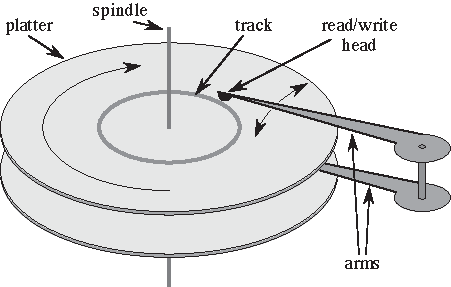
\includegraphics[width=\columnwidth]{images/disk}
				\end{figure}
			\end{column}
			\begin{column}{.6\textwidth}
				\begin{itemize}
					\item Because of the moving mechanical parts, HDD's are slow.
%					\item On average, we need to wait half a turn.
%					\item Moving the arm also takes time.
					\item SSD's are not mechanical, but still significantly slower dan RAM.
					\pause \item[]\(\rightarrow\) \underline{latency}!
				\end{itemize}
			\end{column}
		\end{columns}
	\end{frame}

	\begin{frame}{Combating latency}
		\begin{itemize}[<+->]
			\item Access not just one item, but several at a time.
			\begin{itemize}
				\item Information is divided into a number of equal-sized \textit{blocks}.
				\item B-trees are a very common datastructure for handling this.
			\end{itemize}
			\item Each node is usually as large as a whole disk block.
			\item Reading/writing in secondary memory \(\leftrightarrow\) operations on a B-tree
			\begin{itemize}[<+->]
				\item The number of blocks read or written provides a good approximation of the total time spent accessing the disk drive.
				\item Only downward paths.
				\item So we want the \underline{height} to be \underline{as small as possible}.
			\end{itemize}
		\end{itemize}
	\end{frame}

	\section{Height of a B-tree}

	\begin{frame}{Height of a B-tree}
		\begin{columns}[c]
			\begin{column}{.5\textwidth}
				\onslide<+->\begin{theorem}
					If \(n \geq 1\), then for any \(n\)-key B-tree T of height \(h\) and minimum degree \(t\geq 2\) \[h \leq \log_t\left(\frac{n+1}{2}\right)\]
				\end{theorem}
			\end{column}
			\begin{column}{.5\textwidth}
				\onslide<+->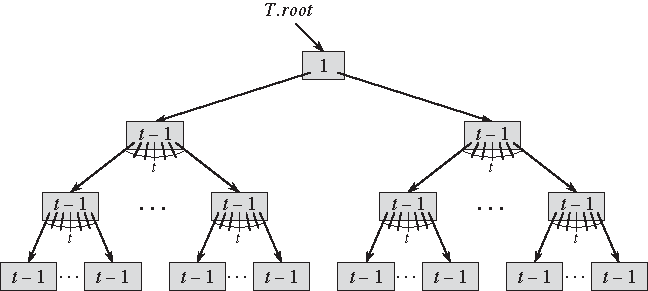
\includegraphics[width=\columnwidth]{images/height}
			\end{column}
		\end{columns}
		\centering
		\vspace{0.5cm}
		\renewcommand*{\arraystretch}{1.4}
		\onslide<+->\begin{tabular}{r | *{6}{|c}}
			depth & \(0\) & \(1\) & \(2\) & \(3\) & ... & \(h\)\\ \hline
			number of nodes & \(1\) & \(2\) & \(2t\) & \(2t^2\) & ... & \(2t^{h-1}\)
		\end{tabular}
	\end{frame}

	\begin{frame}{Height of a B-tree}
		\begin{columns}[c]
			\begin{column}[c]{.55\textwidth}
				\onslide<+->{\textit{Proof.}} \onslide<+->The number of keys \(n\) satisfies \vspace{-0.3cm} \begin{align*}
					n &\geq \overbrace{\underbrace{1}_{\text{root}} + \underbrace{(t-1)}_\text{other nodes}}^{\text{keys per node}} \overbrace{\sum_{i=1}^{h} 2t^{h-1}}^{\text{\#nodes}} \\
					\onslide<+->{& = 1 + 2(t-1)\left(\frac{t^h-1}{t-1}\right)}\\
					\onslide<+->{&= 2t^h-1}
				\end{align*}
				\onslide<+->Thus
				\\ \(
					t^h \leq \dfrac{n+1}{2}\onslide<+-> \Longleftrightarrow \boxed{h \leq \log_t\left(\frac{n+1}{2}\right)}
				\)
				\qed
			\end{column}
			\begin{column}{.45\textwidth}
				\vspace{-0.8cm}
				\onslide<1-6>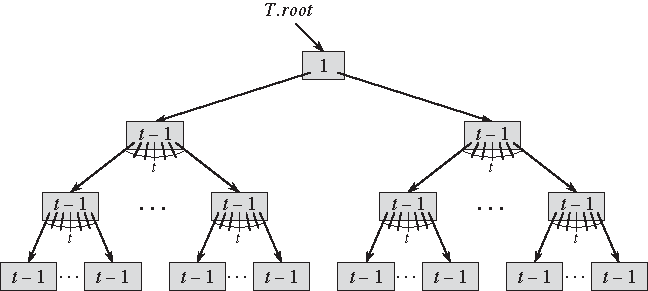
\includegraphics[width=\columnwidth]{images/height}
				\vspace{-0.4cm}
				\begin{table}[h!]
					\begin{tabular}{c | c}
						depth & \#nodes \\ \hline
						\(0\) & \(1\) \\
						\(1\) & \(2\) \\
						\(2\) & \(2t\) \\
						\(3\) & \(2t^2\) \\
						\(\vdots\) & \(\vdots\) \\
						\(h\) & \(2t^{h-1}\)
					\end{tabular}
				\end{table}
			\end{column}
		\end{columns}
	\end{frame}

	\begin{frame}{Comparison with red-black trees}
		\begin{itemize}[<+->]
			\item Height of the tree grows as \(O(\lg n)\) in both cases.
			\begin{itemize}[<+->]
				\item Constant \(t\) is left out in asymptotic notation.
				\item The base logarithm for B-trees is much larger: \(t\) vs \(2\).
			\end{itemize}
			\item Factor of \(\approx \lg t\) saved over red-black trees.
			\item B-trees are \underline{limited in depth} but contain an \underline{enourmous amount of keys}.
			\begin{itemize}
				\item[\(\rightarrow\)] \underline{Few memory operations}, so \underline{minimal memory latency}.
			\end{itemize}
		\end{itemize}
	\end{frame}

	\section{Operations on B-trees}

	\begin{frame}{Searching a B-tree}
		\begin{itemize}[<+->]
			\item \textsc{B-Tree-Search} is much like searching a binary tree.
			\item However, \textit{multiway} (as opposed to binary) branching decisions are made.
			\begin{itemize}[<+->]
				\item The amount of \textit{ways} is equal to the number of children.
				\item At each internal node \(x\), the search makes an \((x.n+1)\)-way branching decision.
			\end{itemize}
			\item Example: searching for the letter \(S\) using lexicographic order. \vspace{0.2cm}\\
			\centering
			\hspace{1cm}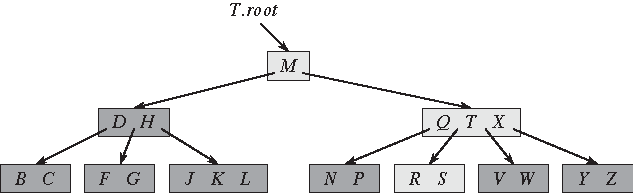
\includegraphics{images/letters}
		\end{itemize}
	\end{frame}

	\begin{frame}{Searching a B-tree: pseudocode}
		\vspace{0.5cm}
		\begin{columns}[c]
			\begin{column}[c]{.5\textwidth}
				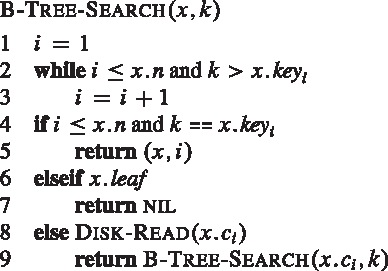
\includegraphics[width=.9\columnwidth]{images/search}
			\end{column}
			\begin{column}[c]{.5\textwidth}
				\pause\begin{itemize}[<+->]
					\item \(x\) is a pointer to the root node of a subtree
					\item \(k\) is the key to be searched
					\item If \(k\) is in the B-tree, \textsc{B-Tree-Search} returns the node-index pair \((y,i)\) such that \(y.key_i=k\). Otherwise, the procedure returns \textsc{nil}.
				\end{itemize}
			\end{column}
		\end{columns}
	\end{frame}

	\begin{frame}{Searching a B-tree: memory access analysis}
		\begin{itemize}[<+->]
			\item The nodes encountered during the recursion form a simple path downward from the root to the tree.
			\item Thus, \textsc{B-Tree-Search} executes \(O(h) = O(\log_t n)\) memory accesses.
			\begin{itemize}[<+->]
				\item Recall that \(h \leq \log_t\left( \frac{n+1}{2}\right) \).
				\item Constants are left out in \(O\)-notation.
			\end{itemize}
		\end{itemize}
	\end{frame}

	\begin{frame}{Searching a B-tree: runtime analysis}
		\vspace{1cm}
		\begin{columns}[c]
			\begin{column}{.5\textwidth}
				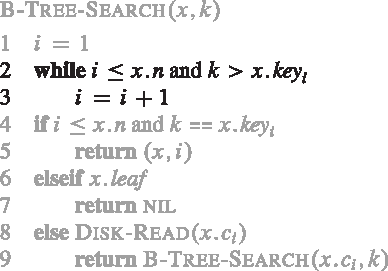
\includegraphics[width=.9\columnwidth]{images/runtime}
			\end{column}
			\begin{column}{.5\textwidth}
				\begin{itemize}[<+->]
					\item For every node \(x\), \(x.n < 2t\), so the while loop takes \(O(t)\) time for each encountered node.
					\item The total runtime is \(O(th)=O(t \log_t n)\).
				\end{itemize}
			\end{column}
		\end{columns}
	\end{frame}

	\begin{frame}{Inserting a key}
		\begin{itemize}[<+->]
			\item Significantly more complicated than inserting a key into a binary tree.
			\item We \underline{cannot simply \textit{create} a new leaf node} and insert it, because the resulting tree would fail to be a valid B-tree.
			\item So, we need to \underline{insert} the key into an \textit{existing} leaf node.
			\item What if a node \(y\) is \textit{full}, i.e. what if \(y.n = 2t-1\)?
		\end{itemize}
	\end{frame}

	\begin{frame}{Splitting a full node \(y\) with \(y.n = 2t-1\)}
		\centering
		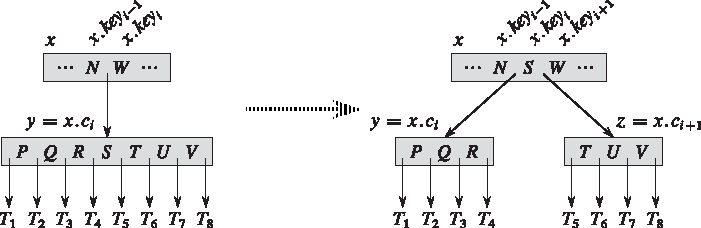
\includegraphics[width=.7\textwidth]{images/splitting}
		\vspace{0.3cm}

		\raggedright
		\onslide<+->\textsc{B-Tree-Split-Child}\((x,i)\)
		\begin{itemize}
			\item \(x\) is a non-full node and \(y=x.c_i\) is a full child of \(x\).
			\item Split \(y\) about its median key \(S\) and move \(S\) up into \(y\)'s parent node \(x\).
			\item Every key \(y.key_i\) that is greater than the median \(S\), is placed in a new node \(z\), which is a new child of \(x\).
		\end{itemize}
	\end{frame}

	\begin{frame}{Inserting a key (continued)}
		Complexity of \textsc{B-Tree-Insert}\((T,k)\)?
%			\begin{itemize}[<+->]
%				\item Checks if the root \(r=T.root\) is full. If it is: \begin{itemize}
%				\item Make the current root child of a new empty root \(s\).
%				\item Splits the old root by calling \textsc{B-Tree-Split-Child}\((s,1)\).
%			\end{itemize}
%			\item Calls \textsc{B-Tree-Insert-Nonfull}\((x,k)\) with either \(x=r\) or \(x=s\)
%			\vspace{0.6cm}
%		\end{itemize}
		\pause
		\begin{itemize}[<+->]
			\item Again \(O(h) = O(\log_t n)\) disk accesses.
			\item Again \(O(th)=O(t \log_t n)\) time required.
		\end{itemize}
	\end{frame}

%	\section{Conclusion}
%
%	\begin{frame}{Conclusion}
%		\begin{itemize}[<+->]
%			\item B-trees are self-balancing data structures optimized for minimizing memory accesses.
%			\item Their logarithmic height and multiway branching make them well-suited for handling large datasets stored in secondary memory.
%			\item Operations like search, insertion, and deletion are efficient, with time complexity \(O(t \log_t n)\) for disk accesses.
%			\item By using nodes as large as disk blocks, B-trees combat latency by reducing the number of required disk reads and writes.
%			\item B-trees are a popular choice for databases.
%		\end{itemize}
%	\end{frame}

	\begin{frame}[c]
		\centering \large Questions?
	\end{frame}


\end{document}
